% !TeX encoding = UTF-8
% Use XeLaTeX to compile it

\documentclass[a4paper,12pt]{book}

\RequirePackage{polyglossia}
 \setdefaultlanguage{russian}
 \setotherlanguage{english}

\RequirePackage{fontspec}
 \setmainfont{CMU Serif}
 \setsansfont{CMU Sans Serif}
 \setmonofont{CMU Typewriter Text}

\RequirePackage{hyperref}
\hypersetup{
	colorlinks
}

\RequirePackage[usenames,dvipsnames]{xcolor}
\RequirePackage{graphicx}
\RequirePackage{wrapfig}
\RequirePackage{textpos}
\RequirePackage{perpage}
\MakePerPage{footnote}

\RequirePackage{geometry}
\geometry{
	a4paper,
	left=35mm,
	right=25mm,
	top=30mm,
	bottom=30mm,
}

\renewcommand{\baselinestretch}{1.15}
\newcommand*{\btw}[1]{\vspace{10pt}\emph{#1}\vspace{10pt}}
\newcommand*{\note}[1]{
	\vspace{12pt}
	\textcolor{Mahogany}{\textbf{\large#1}}
}

\title{Snake Wrangling for Kids - Learning to Program with Python}
\author{Jason R Briggs}

\makeindex
\newcommand{\code}{\textcolor{OliveGreen}\bfseries}
\newenvironment{listing}
{\begin{list}{}{\setlength{\leftmargin}{1em}}\item\footnotesize\samepage}
{\end{list}}
\definecolor{PaleBlue}{rgb}{0.95,0.95,1}


\begin{document}
\pagestyle{empty}
\frontmatter
\begin{titlepage}
\begin{textblock*}{210mm}(-30mm,0mm)
   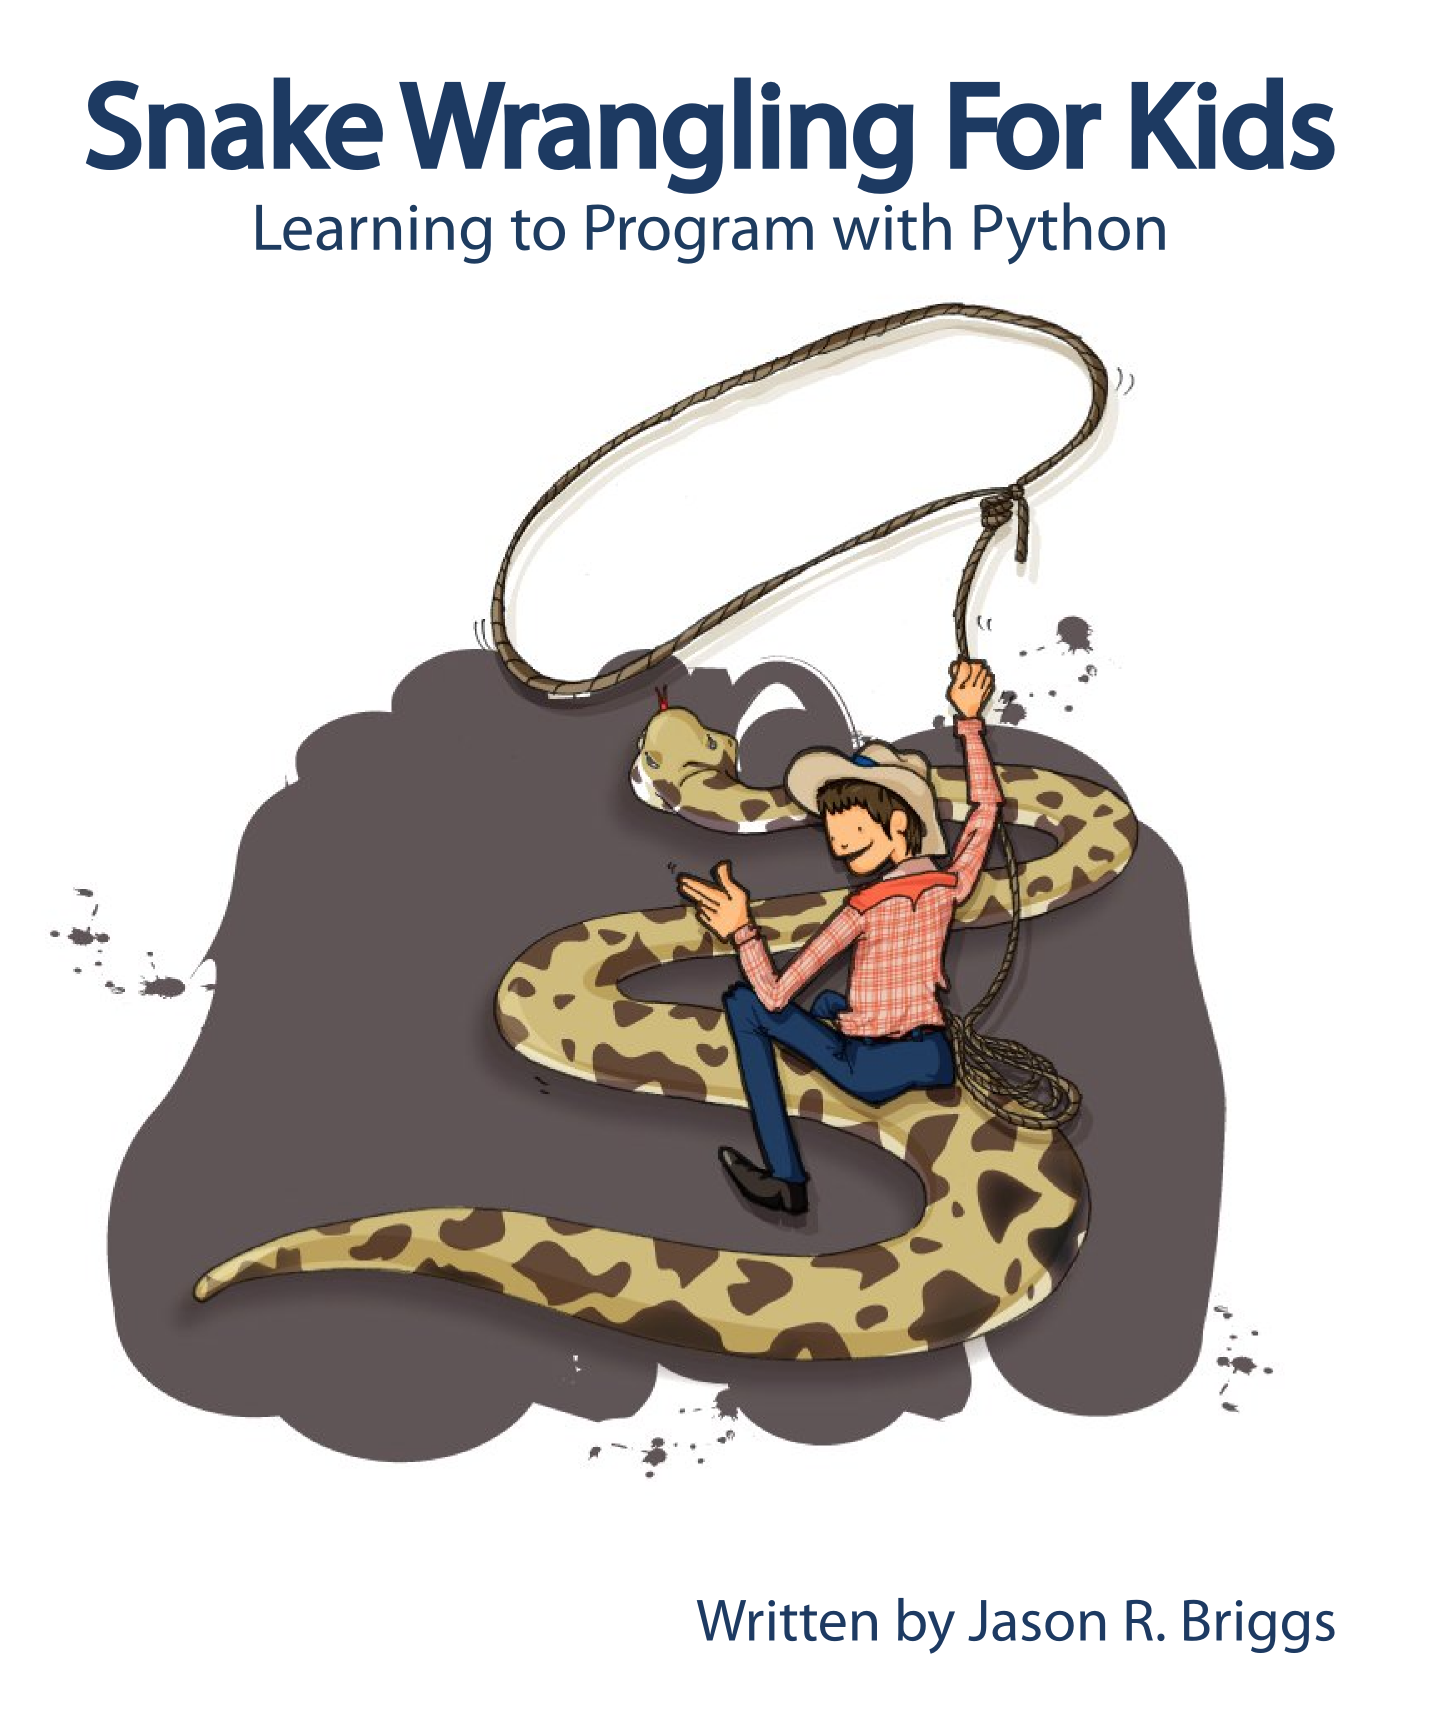
\includegraphics[width=0.9\paperwidth]{../en/cover.eps}
\end{textblock*}
\begin{flushright}
\vspace{30mm}
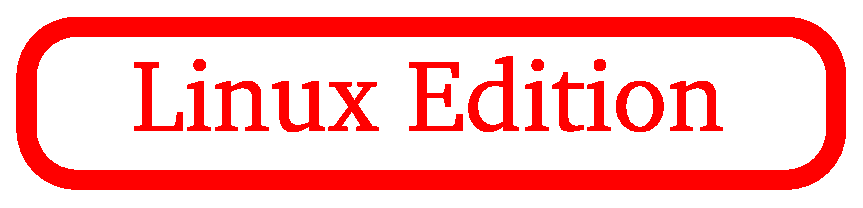
\includegraphics[width=40mm]{../en/linux-edition.eps} 
\end{flushright}
\end{titlepage}

\noindent
\textsf{\emph{Snake Wrangling for Kids, Learning to Program with Python}}\\
by Jason R. Briggs\\
перевод на русский:\\
Кочетов Е.\,М. <Egor.Kochetoff@gmail.com>\\
\\
Version 0.7.7
\\\\
Copyright \copyright 2007.\\
\\
Cover art and illustrations by Nuthapitol C.\\
\\
\noindent
\textsf{\emph{This book has been completely rewritten and updated, with new chapters (including developing graphical games), and new code examples. It also includes lots of fun programming puzzles to help cement the learning. Published by No Starch Press - available here: \href{http://nostarch.com/pythonforkids}{Python for Kids}. Also find more info \href{http://jasonrbriggs.com/python-for-kids/}{here}.}}
\\
\\
\linebreak
\noindent
Website:\\ \href{http://www.briggs.net.nz/log/writing/snake-wrangling-for-kids}{http://www.briggs.net.nz/log/writing/snake-wrangling-for-kids}\\ 
\\
\noindent
Thanks To:\\
Guido van Rossum (for benevolent dictatorship of the Python language), the members of the \href{http://www.python.org/community/sigs/current/edu-sig/}{Edu-Sig} mailing list (for helpful advice and commentary), author \href{http://www.davidbrin.com/}{David Brin} (the original \href{http://www.salon.com/tech/feature/2006/09/14/basic/}{instigator} of this book), Michel Weinachter (for providing better quality versions of the illustrations), and various people for providing feedback and errata, including: Paulo J. S. Silva, Tom Pohl, Janet Lathan, Martin Schimmels, and Mike Cariaso (among others).  Anyone left off this list, who shouldn't have been, is entirely due to premature senility on the part of the author.\\

\noindent
License:\\
\\

\includegraphics[width=40mm]{../en/by-nc-sa.eps}\\
This work is licensed under the Creative Commons Attribution-Noncommercial-Share Alike 3.0 New Zealand License. To view a copy of this license, visit\\ \href{http://creativecommons.org/licenses/by-nc-sa/3.0/nz/}{http://creativecommons.org/licenses/by-nc-sa/3.0/nz/} or send a letter to Creative Commons, 171 Second Street, Suite 300, San Francisco, California, 94105, USA.\\

\noindent
Below is a summary of the license.\\

\noindent
You are free:
\begin{itemize}
 \item \textbf{to Share} — to copy, distribute and transmit the work 
 \item \textbf{to Remix} — to adapt the work
\end{itemize}
\noindent
Under the following conditions:
\begin{description}
 \item[Attribution.] You must attribute the work in the manner specified by the author or licensor (but not in any way that suggests that they endorse you or your use of the work).
 \item[Noncommercial.] You may not use this work for commercial purposes.
 \item[Share Alike.] If you alter, transform, or build upon this work, you may distribute the resulting work only under the same or similar license to this one.
\end{description}

\noindent
For any reuse or distribution, you must make clear to others the license terms of this work.\\

\noindent
Any of the above conditions can be waived if you get permission from the copyright holder.\\

\noindent
Nothing in this license impairs or restricts the author's moral rights.\\

\vspace*{4cm}
\begin{center}

\includegraphics[width=5cm]{../en/python-powered.eps}
\end{center}

\mainmatter

\pagestyle{plain}

\pagenumbering{roman}
\tableofcontents
% preface.tex
% This work is licensed under the Creative Commons Attribution-Noncommercial-Share Alike 3.0 New Zealand License.
% To view a copy of this license, visit http://creativecommons.org/licenses/by-nc-sa/3.0/nz
% or send a letter to Creative Commons, 171 Second Street, Suite 300, San Francisco, California, 94105, USA.


\chapter*{Вступление}\normalsize
    \addcontentsline{toc}{chapter}{Вступление}
\begin{center}
{\em Пара слов для родителей...}
\end{center}
\pagestyle{plain}

Уважаемый родитель или иной управляющий компьютером!

Чтобы ваш ребёнок смог начать знакомиться с программированием, вам нужно установить Python на компьютер. Эта книга была недавно обновлена до версии Python 3.0, самой новой и несовместимой с предыдущими, так что если у вас установлена более старая версия Pyhton, вам стоит скачать и более старую версию этой книги.

Установка Python — достаточно простая задача, но есть несколько тонкостей — в зависимости от используемой операционной системы. Если вы только что купили сверкающий новый компьютер и не имеете никаких идей, что с ним делать, а предыдущее предложение начало вызывать у вас нервную дрожь или холодный пот, то, пожалуй, лучше вам найти кого-то кто сделает это за вас. Установка Python может занять от 15 минут до пары часов в зависимости от скорости интернета и компьютера.

Прежде всего, скачайте и установите последнюю версию Python 3 для вашего дистрибутива. Дистрибутивов очень много, так что инструкции для всех тут привести не получится… да и скорее всего, если вы используете Linux, то уже знаете, как это сделать. Наверное, вы даже возмущены самой идеей того чтобы рассказывать вам, как что-либо устанавливать, так что тут я остановлюсь.

\note{После установки…}

…Вам, возможно, придётся в течение первых пары глав посидеть с ребёнком рядом, но после нескольких примеров ему будет только приятнее читать книгу самому (с компьютером вместе). Нужно рассказать ребёнку, как вводить команды в консоль, как пользоваться текстовым редактором (наподобие блокнота; Microsoft Word никак не подойдёт), открывать и сохранять файлы в этом редакторе. Всё остальное расскажет эта книга.

\vspace{12pt}
\noindent
Спасибо за уделённое время; с наилучшими пожеланиями,\\
КНИГА.


\pagenumbering{arabic}
\pagestyle{headings}
% !TeX encoding = UTF-8
% Use XeLaTeX to compile it
%
% Эта работа распространяется на условиях лицензии Creative Commons Attribution-Noncommercial-Share Alike 3.0 New Zealand License.
% Краткое описание лицензии есть тут: http://creativecommons.org/licenses/by-nc-sa/3.0/nz/deed.ru
% Полное — там же.
% Эту книгу можно невозбранно распространять и изменять, но только соблюдая следующие условия:
% сохраняя лицензию и не вводя дополнительных ограничений, бесплатно
% и указывая авторство как оригинальной части, так и изменённой.
% Автор оригинального английского текста — Jason R Briggs http://jasonrbriggs.com/
% Автор перевода — Егор Кочетов <Egor.Kochetoff@gmail.com>
%
% This work is licensed under the Creative Commons Attribution-Noncommercial-Share Alike 3.0 New Zealand License.
% To view a copy of this license, visit http://creativecommons.org/licenses/by-nc-sa/3.0/nz
% or send a letter to Creative Commons, 171 Second Street, Suite 300, San Francisco, California, 94105, USA.
%

\chapter{Не все змеи будут шипеть на тебя}\label{ch:notallsnakeswillsquishyou}

Возможно, тебе подарили эту книгу на день рожденья. А может, на рождество. Например, так: тётя Агата (у всех есть тётя Агата, но не все об этом знают) хотела подарить носки, хотя и не парные, но оба красивые, на два размера больше — на вырост (и всё равно бы эти носки не пригодились потом). А потом вместо этого услышала про эту книгу (которую можно взять и напечатать), вспомнила твои вопросы про всякие компьютерные штуки, и твои непонятные объяснения, как пользоваться компьютером, оборвавшиеся в момент, когда она начала разговаривать с компьютерной мышью, и решила подарить эту книгу. Во всяком случае эта книга уж точно лучше пары разных носков.

Надеюсь, я не слишком тебя разочаровываю тем, что я — возможно, напечатанная на какой-нибудь старой обёрточной бумаге (хотя если повезло, то и нет) — не слишком разговорчивая (прямо, скажем, совсем молчаливая) книга, с пугающим словом «изучение» в названии... Но представь на минутку и мои ощущения. Если бы вот ты был персонажем из какой-нибудь книги про волшебников, одна из которых наверняка есть у тебя в спальне на книжной полке, — у меня бы могли быть зубы... или даже глаза! А ещё какие-нибудь движущиеся картинки, таинственные звуки... ладно, чего я. В общем, я просто бумажная книжка, хотя могло бы быть и лучше.

\btw{Ах, много бы я дала за пару хороших острых челюстей...}

Но вообще, быть конкретно такой книжкой тоже не слишком печально. Ну не могу я говорить... пальцы покусывать не могу; зато могу рассказать немного о том, что заставляет компьютеры работать. Не про разные аппаратные штуки — все эти провода, платы, чипы — они меня немного пугают. Электричеством, например, могут ударить (так что не стоит и пытаться туда лезть, как по мне). Я могу рассказать о том, что удивительным образом скрыто внутри всех этих проводов, микросхем и что делает компьютер по-настоящему полезным.

\begin{wrapfigure}{r}{0.5\textwidth}
  \begin{center}
\includegraphics*[width=70mm]{../en/electrocute.eps}
  \end{center}
\end{wrapfigure}

Вообще, это здорово похоже на мысли, например, в твоей голове. Если бы мыслей у тебя не было — сидел бы ты, скажем, на полу в спальне и бессмысленно смотрел в пространство перед собой. Без \emph{программ} компьютеры бы могли приносить пользу, пожалуй, разве что как стопор для двери. Да и то посредственный: вечно все бы об него спотыкались по ночам. А что может быть хуже, чем удариться ночью в темноте пальцем ноги с размаху о железный угол...

\btw{Итак, я всего лишь книга. И мне это хорошо известно.}

Вообще, у тебя в семье могут быть разные устройства вроде Playstation, Xbox, Wii — игровые консоли, — а ещё DVD-проигрыватель, может, даже современный холодильник и игрушечная машинка. В них во всех есть программы, которые делают их намного полезнее, чем если бы эти штуки были без программ. В DVD-проигрывателе есть программа для чтения и воспроизведения дисков. В холодильнике — какая-то простая программа для поддержания температуры при минимальных затратах электричества. В машинке — программа для приёма команд с пульта управления и для езды в ответ на эти команды. А в настоящих машинах программы показывают маршруты в объезд пробок и сигналят водителю, когда он паркуется, чтоб он никуда не въехал (в стену или соседнюю машину).

Зная, как писать программы, ты сможешь сделать множество самых разных полезных вещей. Можно свою игру написать. Можно писать страницы в интернете, которые что-нибудь делают, а не просто показывают текст и картинки. Можно упрощать себе выполнение домашней работы.

Так вот, пора приступить к чему-то чуть более интересному, чем эти рассуждения.

\section{Пара слов про язык}

Так же как и у людей, определённо как у китов, возможно, и у дельфинов и, возможно, у родителей (тут, конечно, спорно), у компьютеров есть свой собственный язык. Вообще, как и у людей, у компьютеров много языков. Какую букву английского алфавита ни возьми, она называет какой-нибудь язык. Вот, например, буквы A, B, C, D, E — не только буквы, но и названия языков программирования (что ещё раз доказывает, что у взрослых никакого воображения и хорошо бы им давать почитать хотя бы словарь перед тем, как названия придумывать).

Есть ещё языки программирования, названные в честь людей\footnote{например, язык Ада — в честь \href{https://ru.wikipedia.org/wiki/\%D0\%9B\%D0\%B0\%D0\%B2\%D0\%BB\%D0\%B5\%D0\%B9\%D1\%81,_\%D0\%90\%D0\%B4\%D0\%B0}{Ады Лавлейс}. А есть ещё язык \href{https://ru.wikipedia.org/wiki/\%D0\%A3\%D1\%87\%D0\%B5\%D0\%B1\%D0\%BD\%D1\%8B\%D0\%B9_\%D0\%B0\%D0\%BB\%D0\%B3\%D0\%BE\%D1\%80\%D0\%B8\%D1\%82\%D0\%BC\%D0\%B8\%D1\%87\%D0\%B5\%D1\%81\%D0\%BA\%D0\%B8\%D0\%B9_\%D1\%8F\%D0\%B7\%D1\%8B\%D0\%BA}{РАЯ}.},
есть языки-сокращения из заглавных букв (SQL, например),  есть немножко названных в честь телевизионных шоу. А, да, ещё если дописать к этим буквам всяких значков типа плюсиков, решёточек (+, \#), то тоже получатся названия разных языков программирования. И ещё впридачу некоторые языки очень похожи и отличаются только в каких-то мелочах.

\btw{Что я говорила? Никакого воображения!}

К счастью, многие из языков уже почти не используются или совсем исчезли; но однако же список способов «говорить» с компьютером всё ещё пугающе велик. Я буду обсуждать только один из них, потому что иначе всё так и закончится их перечислением, не успеем мы приступить к чему-то действительно интересному.

\section{Орден Неядовитых Удушающих Змей...}

... или просто питонов.

Вообще, питон — не только змея\footnote{которая \href{https://ru.wikipedia.org/w/index.php?title=\%D0\%9F\%D0\%B8\%D1\%82\%D0\%BE\%D0\%BD\%D1\%8B&oldid=70828612\#.D0.9F.D0.B8.D1.82.D0.B0.D0.BD.D0.B8.D0.B5}{может} не есть полтора года кряду!}, но и язык программирования. Многие называют его «пайтон», как принято за рубежом, где его и придумали (и пишут его название как Python). Язык, правда, был назван не в честь змеи — это один из немногих языков программирования, названных в честь телевизионного шоу. \href{http://www.youtube.com/watch?v=YO2xZbac7lw&list=PL89E217812DCA2BDA}{Монти Пайтон} (Monty Python) — \href{http://www.montypython.com/}{британское телешоу}, популярное с 1970х годов. Требуется достичь некоторого возраста и иметь определённый склад ума, чтобы счесть его забавным, но многим нравится. Хотя лет до 12 смотреть вообще смысла нет, будет скучно и непонятно.

Есть несколько особенностей Питона (языка программирования, а не змеи), делающих его очень полезным, чтобы учиться программировать. Для нас сейчас важнее всего то, что используя его, можно быстро сесть и начать писать какие-то программки, пусть и очень простые, без долгих разговоров и объяснений.

Это тот момент, когда надо убедиться, что твоя мама, папа или кто там управляет компьютером прочли часть «Заметка для мам и пап». Есть хороший способ проверить это. Спроси у них, как называется программа-\emph{эмулятор терминала} — это может быть \texttt{yakuake}, \texttt{konsole}, \texttt{rxvt}, \texttt{xterm} или ещё какая-нибудь, их очень много бывает — именно поэтому придётся спросить. Запусти эту программу, напиши \emph{в командной строке} «python3» (без кавычек) и нажми на клавиатуре клавишу Enter. На экране должно появиться что-то похожее на рисунок \ref{fig4}.

\begin{figure}
\begin{center}
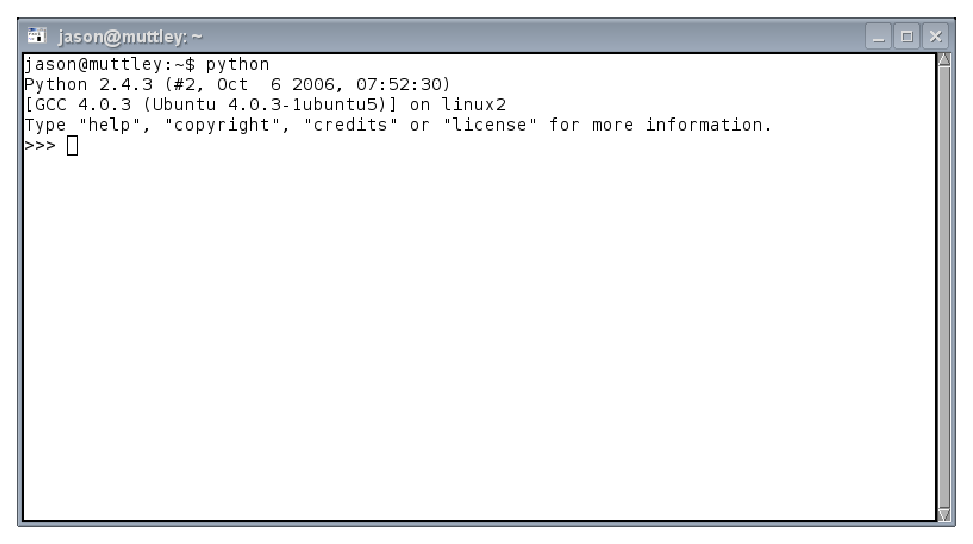
\includegraphics[width=80mm]{../en/figure4.eps}
\end{center}
\caption{Консоль Питона в Линуксе.}\label{fig4}
\end{figure}

\begin{samepage}
\note{Если ты обнаружишь, что они не прочитали инструкции в начале книги...}
\nopagebreak
\paragraph*{}
... и из-за этого у тебя не получилось что-то сделать, то перелистни эту книгу на начало, подсунь им под нос введение, пока они читают утреннюю газету, и умоляюще посмотри на них. Иногда помогает говорить «пожалуйста-пожалуйста-пожалуйста» до тех пор, пока они не встанут и не сделают всё, что надо. Ну и конечно, можно попробовать сделать всё самостоятельно, это может оказаться даже проще.
\end{samepage}

\section{Первая программа на Питоне}

Так или иначе, если ты добрался досюда, у тебя уже открыта \emph{консоль}, или командная строка Питона — это один из способов запускать команды и целые программы на Питоне. После запуска консоли или ввода любой команды ты увидишь \emph{приглашение командной строки}, которое в Питоне выглядит вот так:

\begin{verbatim}
>>>
\end{verbatim}

Если записать несколько команд на Питоне одну за другой, получится программа, которую можно запускать и не через консоль, но пока на минутку остановимся на простых командах, которые можно вводить прямиком в командную строку (после «приглашения»). Например, можно ввести туда следующую команду:

\begin{verbatim}
print("Всем привет!")
\end{verbatim}

Чтобы всё получилось, нужно ввести и скобки и кавычки (вот эти: "") так, как написано выше. Тогда на экране должно появиться что-то вроде такого:

\begin{verbatim}
>>> print("Всем привет!")
Всем привет!
\end{verbatim}

После этого приглашение командной строки появится снова, чтобы показать, что Питон готов принимать новые команды. Поздравляю! Ты только что создал и запустил свою первую программу на Питоне — пусть пока и всего из одной команды: print — функции, которая просто печатает всё, что написано в скобках. Потом мы много будет использовать эту команду.

\section{Вторая программа на питоне… опять то же самое?}

Программы на Питоне были бы не слишком полезными, если бы их приходилось каждый раз вводить заново в командную строку или если бы ты написал программу для кого-то, а ему бы пришлось её перепечатывать, чтобы запустить.

Программа для редактирования текстов (Microsoft Word, Libreoffice Writer или другая подобная), которую ты, вероятно, используешь для выполнения каких-нибудь домашних заданий, получена из исходного кода размером примерно от 10 до 100 миллионов строк. Если печатать это на бумаге с двух сторон не очень крупно, это может занять, например, 400 000 страниц. Это стопка бумаги высотой 40 метров, с десятиэтажный дом. Такое количество бумаги нести из магазина в дом, чтобы перепечатать, пришлось бы долго… очень долго…

…а если бы ещё и ветер подул в подходящий момент… за бумагой пришлось бы долго бегать. Так вот, хорошая новость: всем этим заниматься не обязательно.

\begin{center}
\includegraphics*[width=85mm]{../en/pullinghair.eps}
\end{center}

Открой текстовый редактор (можешь опять спросить у родителей, как он называется: например, kate, gedit, kdevelop, но никак не Microsoft Word, он не подойдёт) и напиши туда точно ту же самую команду, что ты до этого вводил в консоль:

\begin{verbatim}
print("Всем привет!")
\end{verbatim}

%todo save.png
Теперь сохрани этот файл в своей домашней папке. Наверху в программе должен быть значок сохранения, а когда тебя спросят, куда сохранять, нажми на какую-нибудь кнопку типа домика. В качестве имени файла введи «hello.py». Теперь опять открой терминал и напиши:

\begin{verbatim}
python hello.py
\end{verbatim}

В консоли должно появиться приветствие от программы, точно так же, как в прошлый раз (примерно как на рисунке \ref{fig9}).

\begin{figure}
\begin{center}
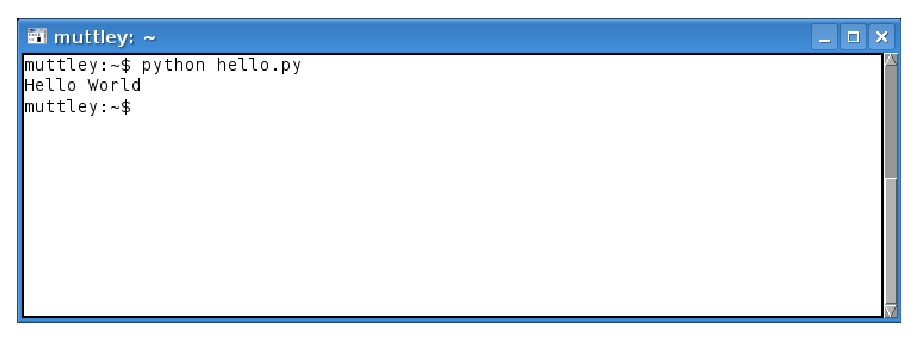
\includegraphics[width=75mm]{../en/figure9.eps}
\end{center}
\caption{Запуск программы на Питоне, сохранённой в текстовый файл}\label{fig9}
\end{figure}

Вот. Теперь ты видишь, что мудрые люди, создавшие Питон, спасли тебя от ввода одних и тех же программ много-много-много раз для выполнения одних и тех же действий. Как они делали в 1980х. Я серьёзно, им приходилось вводить каждый раз кучу команд для выполнения одной и той же программы. Можешь спросить у папы — вдруг у него был ZX81 в молодости — так там приходилось так делать. Теперь можно просто написать имя программы, и она целиком исполнится от начала до конца.

\note{Конец начала}

Добро пожаловать в удивительный мир программирования!
Мы начали с простой программы, которая печатает «Всем привет» («Hello world») — все с этого начинают, когда учатся программировать. В следующей главе мы займёмся чуть более полезными вещами в консоли Питона, а потом изучим, как написать программу посложнее.

% !TeX encoding = UTF-8
% Use XeLaTeX to compile it
%
% Эта работа распространяется на условиях лицензии Creative Commons Attribution-Noncommercial-Share Alike 3.0 New Zealand License.
% Краткое описание лицензии есть тут: http://creativecommons.org/licenses/by-nc-sa/3.0/nz/deed.ru
% Полное — там же.
% Эту книгу можно невозбранно распространять и изменять, но только соблюдая следующие условия:
% сохраняя лицензию и не вводя дополнительных ограничений, бесплатно
% и указывая авторство как оригинальной части, так и изменённой.
% Автор оригинального английского текста — Jason R Briggs http://jasonrbriggs.com/
% Автор перевода — Егор Кочетов <Egor.Kochetoff@gmail.com>
%
% This work is licensed under the Creative Commons Attribution-Noncommercial-Share Alike 3.0 New Zealand License.
% To view a copy of this license, visit http://creativecommons.org/licenses/by-nc-sa/3.0/nz
% or send a letter to Creative Commons, 171 Second Street, Suite 300, San Francisco, California, 94105, USA.
%

\chapter{8 умножить на 3.57 равняется…}\label{ch:8multipliedby3.57}

Чему равно 8 умножить на 3.57? Пришлось бы использовать калькулятор, чтобы посчитать? Ладно, этот пример можно вычислить и в уме, но не в том дело. То же самое можно сделать в консоли Питона. Запусти её опять (как описано в предыдущей главе), если она ещё не запущена, и введи туда такую команду: \texttt{8*3.57}. Потом нажми Enter.

\begin{verbatim}
Python 3.4.0 (default, Apr 11 2014, 13:05:11) 
[GCC 4.8.2] on linux
Type "help", "copyright", "credits" or "license" for more information.
>>> 8 * 3.57
28.56
\end{verbatim}

Звёздочка (\code{*}) (обычно это shift + 8) используется для умножения\index{умножение} вместо привычного символа $×$ (или $\cdot$), потому что не везде их можно просто так ввести с клавиатуры, а буква X путалась бы с собственно буквой, если бы её использовали как знак умножения. Ладно, как насчёт чего-нибудь более полезного?

Представь, что тебе приходится заниматься делами по хозяйству раз в неделю, за что каждый раз ты получаешь по 5 рублей и ещё у тебя есть курьерская подработка по доставке газет за 30 рублей в неделю. Сколько денег такими темпами накопится за год?

\begin{figure}[t]
\begin{center}
\fbox{\colorbox{PaleBlue}{\parbox{.75\linewidth} {
\subsection*{Питон сломался!?!?}

Если ты возьмёшь калькулятор и введёшь туда \texttt{8×3.57}, ответ на экране будет такой:

\vspace{10pt}
\textsf{28.56}
\vspace{10pt}

В Питоне ответ может быть такой же, а может быть такой:

\vspace{10pt}
\textsf{28.55999999}
\vspace{10pt}

Чем Питон отличается? Уж не поломан ли он??

Да нет, вообще-то. Просто так дробные числа (числа с десятичной запятой, или \emph{числа с плавающей запятой}\index{числа с плавающей запятой}) представляются в компьютере: приближённо. Результаты всегда почти точные, но далеко справа после точки могут набегать небольшие ошибки вычисления после выполнения последовательности действий. Дробные числа представляются в компьютере не очень просто, мы не будем сейчас на этом останавливаться. Я хочу сказать, не удивляйся, что \emph{иногда} результаты вычислений не в точности равны тому, что ты ожидаешь; это верно для умножения, деления, сложения и вычитания.

Целые числа в компьютере представляются точно и всегда вычисляются без ошибок в Питоне (в других языках программирования есть свои хитрости).
}}}
\end{center}
\end{figure}

Если бы мы решали эту задачу на бумаге, то написали бы что-то вроде:

\begin{verbatim}
(5 + 30) × 52
\end{verbatim}

Что значит: (5 руб + 30 руб), умноженное на 52 недели в году.
\begin{samepage}
Можно, конечно, и сразу сократить эту запись до такой:

\begin{verbatim}
35 × 52
\end{verbatim}
\end{samepage}

И это уже совсем просто посчитать что на калькуляторе, что в столбик (в уме сложнее). А можно всё то же самое сделать в консоли:

\begin{listing}
\begin{verbatim}
>>> (5 + 30) * 52
1820
>>> 35 * 52
1820
\end{verbatim}
\end{listing}

Как быть, если ты тратишь 10 рублей в неделю? Что теперь останется к концу года? Можно было бы разными способами записать это на бумаге, но давай опять обратимся к консоли:

\begin{listing}
\begin{verbatim}
>>> (5 + 30 - 10) * 52
1300
\end{verbatim}
\end{listing}

Это значит: 5 рублей и ещё 30 рублей минус 10 потраченных рублей, и всё умножается на 52 недели в году. В конце года будет 1300 накопленных рублей. Ладно, я понимаю, что выглядит это всё не слишком полезно, и без Питона тут было бы легко обойтись. Мы потом опять вспомним про этот пример, и я покажу, как сделать из него куда более полезный.

В питоньей консоли можно умножать\index{умножение}, складывать\index{сложение}, вычитать\index{вычитание} и делить\index{деление}. Можно выполнять и другие арифметические действия, но мы пока их пропустим. Вот так выглядят символы математических операций\index{математические операции}:

\begin{center}
\begin{tabular}{|c|c|}
\hline
$+$ & Сложение \\
\hline
$-$ & Вычитание \\
\hline
$*$ & Умножение \\
\hline
$/$ & Деление \\
\hline
\end{tabular}
\end{center}

Для деления используется косая черта («прямой слэш» или просто «слэш», как его ещё называют), потому что рисовать дроби с клавиатуры не так-то просто, а символа деления ($\div$) обычно тоже нет.

Если бы тебя попросили сказать, сколько коробок, в которые влезает по 20 яиц, нужно для 100 яиц, ты мог бы написать что-то такое:

\begin{displaymath}
\frac{100}{20}
\end{displaymath}

или такое:

\begin{displaymath}
\begin{array}{rr|r}
100&&20\\
\cline{3-3}
100&&5\\
\cline{1-1}
0
\end{array}
\end{displaymath}

ну или, может, такое (хотя так чаще за рубежом пишут)

\begin{displaymath}
100 \div 20
\end{displaymath}

Так вот, в Питоне надо написать вот так: \code{100 / 20}.

\btw{Что, на мой взгляд, гораздо проще. Впрочем, что я в этом понимаю, я всего лишь книга.}

\section{Использование скобок и «приоритет операций»}\index{приоритет операций}

В языках программирования (да и просто в математике) мы используем скобки, чтобы управлять тем, что называется «приоритет операций». Операции не ограничиваются четырьмя арифметическими, бывают и другие, но смысл одинаковый. Из этих четырёх операций умножение и деление, как обычно, выполняются перед сложением и вычитанием, то есть у них выше приоритет. В примере ниже у всех операций одинаковый приоритет, поэтому они все выполняются слева направо:

\begin{listing}
\begin{verbatim}
>>> print(5 + 30 + 20)
55
\end{verbatim}
\end{listing}

В примере ниже тоже у всех одинаковый приоритет, и тоже все операции выполняются по порядку слева направо:

\begin{listing}
\begin{verbatim}
>>> print(5 + 30 - 20)
15
\end{verbatim}
\end{listing}

А вот в следующем примере есть умножение. Тут сначала умножаются числа 20 и 30, а потом к ним прибавляется 5: у умножения выше приоритет.

\begin{listing}
\begin{verbatim}
>>> print(5 + 30 * 20)
605
\end{verbatim}
\end{listing}

Что будет, если добавить скобок? Вот что:

\begin{listing}
\begin{verbatim}
>>> print((5 + 30) * 20)
700
\end{verbatim}
\end{listing}

Почему поменялся результат? Потому что скобки меняют порядок операций. Сначала вычисляется то, что в скобках, а потом всё, что снаружи. Тут сначала к 5 прибавляется 30, а результат всего Питон умножает на 20.

Можно использовать скобки более сложным образом. Можно внутри скобок писать ещё скобки:

\begin{listing}
\begin{verbatim}
>>> print(((5 + 30) * 20) / 10)
70
\end{verbatim}
\end{listing}

Тут Питон сначала вычисляет то, что внутри самых вложенных скобок, потом то, что во внешних скобках, и потом выполняет операцию деления, которая вообще не в скобках (самые внешние скобки нужны слову print, а не чтобы указывать порядок операций). Это выражение можно прочитать так: «прибавь к 5 30, потом это всё умножь на 20 и результат подели на 10». Без скобок всё было бы иначе:

\begin{listing}
\begin{verbatim}
>>> 5 + 30 * 20 / 10
65
\end{verbatim}
\end{listing}

Тут сначала 30 умножается на 20, потом делится на 10 и к этому всему прибавляется 5.

\btw{Помни, что умножение и деление всегда выполняются перед сложением и вычитанием, если только скобки не указывают делать иначе.}

\section{Нет ничего столь же непостоянного, как переменная}\index{переменные}

«Переменная» в программировании — название места для хранения разных штук. «Разные штуки» могут быть числами, текстом, списками чисел или строк и множеством других вещей, о которых обо всех сейчас пока рассказать сложно. Давай пока считать, что переменная — это что-то вроде почтового ящика.

\begin{center}
\includegraphics*[width=76mm]{../en/girlbubble.eps}
\end{center}

В почтовый ящик можно положить что-нибудь: письмо, газету — и в переменную можно точно так же положить что-нибудь: число, строку, список чисел. Именно таким образом работают переменные в большинстве языков программирования: в них что-нибудь кладут. Правда, не во всех языках так.

В Питоне переменные используются немножко иначе. Они не хранят что-то внутри себя, а, скорее, работают наклейкой на почтовом ящике. Эту наклейку можно снять и переклеить на другой ящик, например. А можно прилепить сразу на несколько каких-нибудь коробок (обмотав их предварительно скотчем). В питоне эта операция прилепливания выглядит как знак равенства. Чтобы создать переменную, нужно написать её имя слева от этого знака, а справа — то, на что эта переменная указывает. Например, вот так:

\begin{listing}
\begin{verbatim}
>>> Фёдор = 100
\end{verbatim}
\end{listing}

Мы сейчас создали переменную, называющуюся \code{Фёдор}, и сказали, что она указывает на число 100. Тут мы ещё говорим Питону запомнить это число, потому что собираемся его потом использовать. Чтобы узнать, на что переменная указывает, можно вывести её значение функцией \code{print}, как-то так:

\begin{listing}
\begin{verbatim}
>>> Фёдор = 100
>>> print(Фёдор)
100
\end{verbatim}
\end{listing}

Можно сказать Питону, что \code{Фёдор} теперь должен указывать на другое число:

\begin{listing}
\begin{verbatim}
>>> Фёдор = 200
>>> print(Фёдор)
200
\end{verbatim}
\end{listing}

%TODO уточнить процент лабуды в следующем предложении. Константы реально сборщиком мусора убираются в питоне?
Теперь \code{Фёдор} указывает на число 200 (а число 100, которое больше не нужно, Питон потом забудет, когда оно будет мешать). И \code{print} подтвердил нам, что Фёдор теперь указывает на 200.
Можно наклеить на это же самое 200 и ещё одну наклейку, то есть создать ещё одну переменную, указывающую на него:

\begin{listing}
\begin{verbatim}
>>> Фёдор = 200
>>> Василий = Фёдор
>>> print(Василий)
200
\end{verbatim}
\end{listing}

В этом кусочке кода мы создаём переменную \code{Василий}, которая указывает туда же, куда и \code{Фёдор}. Если Фёдор поменяет своё значение, Василия это не коснётся.

Вообще, конечно, «Фёдор» — не самое подходящее имя для переменной. Обычно имена переменных записывают английскими буквами — так программистам со всего мира гораздо проще читать и дополнять программы друг друга. Ну и кроме того, имя переменной должно бы говорить, зачем она нужна. Вот с почтовым ящиком всё понятно, он нужен, чтобы разную почту хранить. А переменная может хранить совершенно разные вещи, совсем по-разному устроенные, и переменных в программе обычно очень много. Поэтому называть переменную нужно так, чтобы сразу было понятно, для чего она используется\footnote{Некоторые даже считают, что придумывать хорошие имена переменным — самое сложное в работе программиста.}.

Представь себе, что ты открыл консоль Питона, напечатал \code{Фёдор = 200}, а потом отошёл от компьютера. На 10 лет. Чтобы залезть на Эверест, потом пересечь пустыню Сахару, попрыгать с моста на резинке в Новой Зеландии и спуститься на лодках по реке Амазонке. И потом обратно вернулся к консоли. Самое сложное будет понять: почему Фёдор и почему 200?!

Обычно, чтобы всё забыть, хватает гораздо меньшего времени, чем 10 лет. А часто программу пишут сразу несколько людей, каждый из которых не знает мысли остальных. Так что лучше с самого начала называть все переменные понятно и не рассчитывать на свою память.

Так-то! Смотри, например, мы можем назвать переменную так:\\\code{number\_of\_students}.

\begin{listing}
\begin{verbatim}
>>> number_of_students = 200
\end{verbatim}
\end{listing}

Так сделать получится, потому что имена переменных можно составлять из букв, цифр и знаков подчёркивания (главное, чтобы имя не начиналось с цифры). Если ты вернёшься к своему коду через 10 лет, то «number\_of\_students» всё ещё будет иметь смысл (по крайней мере, если ты знаешь английский хоть немного, что в любом случае пригодится). Можно будет напечатать вот так:

\begin{listing}
\begin{verbatim}
>>> print(number_of_students)
200
\end{verbatim}
\end{listing}

И сразу будет понятно, что количество студентов (где-то) — 200. Не всегда есть смысл придумывать длинные осмысленные имена переменных: иногда переменная используется всего в паре строк, иногда можно использовать вообще одну букву в качестве имени, и есть такие случаи, когда всем это будет привычно и понятно. В основном, это зависит от того, захочется ли потом понять по имени переменной, зачем она вообще нужна, или это будет почему-нибудь понятно и без этого.

\begin{listing}
\begin{verbatim}
это_тоже_допустимое_имя_переменной_но_наверное_не_слишком_полезное
\end{verbatim}
\end{listing}

\section{Используем переменные}\index{переменные}

Ладно, как создавать переменные мы разобрались. Но что с ними делать?

А вот что. Помнишь тот пример, который мы считали выше? Сколько денег заработается за год? Вот этот:

\begin{listing}
\begin{verbatim}
>>> print((5 + 30 - 10) * 52)
1300
\end{verbatim}
\end{listing}

Что если нам сюда добавить три переменных? Вот так:

\begin{listing}
\begin{verbatim}
>>> chores = 5
>>> paper_round = 30
>>> spending = 10
\end{verbatim}
\end{listing}

В переменных записано, сколько денег получается за неделю: 5 руб. за домашние дела и 30 — за курьерство — и сколько денег тратится в неделю: 10 рублей. Можно теперь перепечатать тот же пример вот так:

\begin{listing}
\begin{verbatim}
>>> print((chores + paper_round - spending) * 52)
1300
\end{verbatim}
\end{listing}

Ответ такой же. А что если теперь за домашние дела ты будешь получать семь рублей вместо пяти? Надо записать в переменную \code{chores} значение 7, а потом нажать пару раз кнопку вверх на клавиатуре, чтобы появился опять пример на экране, и Enter, вот так:

\begin{listing}
\begin{verbatim}
>>> chores = 7
>>> print((chores + paper_round - spending) * 52)
1404
\end{verbatim}
\end{listing}

Так пришлось гораздо меньше печатать, чтобы получить новый ответ, чем без использования переменных. Можно попробовать поменять другие переменные и опять нажимать клавишу вверх, чтобы получать новые ответы:

\begin{listing}
\begin{verbatim}
Что будет если тратить вдвое больше:
>>> spending = 20
>>> print((chores + paper_round - spending) * 52)
884
\end{verbatim}
\end{listing}

Если тратить 20 рублей в неделю, то к концу года получится накопить только 884 рубля. Пока переменные не сильно много пользы нам принесли, но уже понятно, что с ними проще и что они могут что-нибудь хранить.

\btw{Вспоминай почтовый ящик с наклейкой на нём!}

\section{Кусочек строки}\index{строки}

Если ты уделяешь внимание моим словам, а не просто бегло проглядываешь книжку в поисках интересных картинок, то можешь вспомнить, что я говорила, что в переменных можно хранить разного сорта вещи, а не только числа. Например, можно хранить текст, или, как его обычно называют в программировании, строки (по-английски: \emph{string}). Такое название может поначалу показаться странным, но, если подумать, текст — это просто буквы, составленные в слова, составленные в строки, и ничего больше. Может быть, так понятнее.

\btw{А может, и не понятнее...}

В таком случае, всё, что тебе необходимо знать, — это что строка — не более чем составленные вместе буквы, цифры и любые другие символы. Ну и обычно они что-то значат все вместе. Всё содержимое этой книги можно записать в строку. Твоё имя можно записать строкой. Твой домашний адрес тоже. Мы, кстати, уже использовали строку в первой программе, вот эту: "Всем привет!".

В Питоне строка создаётся просто: нужно поставить кавычки (такие: " или такие: ') вокруг текста. Можно вспомнить про нашу бесполезную переменную Фёдора и записать в неё строку, вот так:

\begin{listing}
\begin{verbatim}
>>> Фёдор = "я маленькая строка"
\end{verbatim}
\end{listing}

И как всегда, можно узнать, что хранит Фёдор:

\begin{listing}
\begin{verbatim}
>>> print(Фёдор)
я маленькая строка
\end{verbatim}
\end{listing}

Или вот пример с одинарными кавычками:

\begin{listing}
\begin{verbatim}
>>> Фёдор = 'и я строка'
>>> print(Фёдор)
и я строка
\end{verbatim}
\end{listing}

\index{многострочная строка}Но если ты попытаешься сохранить в переменную сразу несколько строк текста\footnote{По-английски это называется \emph{multilne string}, то есть «многострочная строка». Строка с переносами строк внутри, иначе говоря.}, используя просто кавычки, то ничего не выйдет. Например, попробуй напечатать команду, написанную ниже, и получишь пугающе непонятное сообщение об ошибке, что-то вроде такого:

\begin{listing}
\begin{verbatim}
>>> Фёдор = "первая строка
  File "<stdin>", line 1
    Фёдор = "первая строка
                          ^
SyntaxError: EOL while scanning string literal
\end{verbatim}
\end{listing}

Про эту ошибку мы поговорим позже, а пока можешь просто запомнить, что чтобы сохранить в переменную сразу несколько строк текста, нужно использовать три одинарных кавычки\footnote{Обычно одинарную кавычку можно ввести только в английской раскладке и она находится на той же клавише, где русская «Э», справа→ на клавиатуре.}:

\begin{listing}
\begin{verbatim}
>>> Фёдор = '''вот строка
... с переносом строки внутри'''
\end{verbatim}
\end{listing}

Напечатай эту переменную, чтобы проверить, что всё получилось:

\begin{listing}
\begin{verbatim}
>>> print (Фёдор)
вот строка
с переносом строки внутри
\end{verbatim}
\end{listing}

Пока ты печатал эту строчку с переносом, то мог обратить внимание, что Питон вместо приглашения на второй строке напечатал три точки (...). Он это делает в тех случаях, когда что-то, начатое на первой строке, продолжается на следующей — вот как строка. Пока кавычки не закроются, Питон так и будет печатать «...», показывая, что ждёт завершения строки. Потом мы и в других случаях увидим эти три точки.

\section{Развлечения со строками}

Вот есть интересный вопрос: чему равно 10 * 5 (10 умножить на 5)? Ответ, конечно: 50.

\btw{Ладно, это был неинтересный вопрос.}

А чему равно 10 * 'а' (10 умножить на букву а)? Вопрос может показаться бессмысленным, но вот ответ от Питона:

\begin{listing}
\begin{verbatim}
>>> print(10 * 'a')
aaaaaaaaaa
\end{verbatim}
\end{listing}

Это работает не только с отдельными символами, но и со строками подлиннее:

\begin{listing}
\begin{verbatim}
>>> print(20 * 'abcd')
abcdabcdabcdabcdabcdabcdabcdabcdabcdabcdabcdabcdabcdabcdabcdabcdabcdabcdabcdabcd
\end{verbatim}
\end{listing}

Есть ещё один трюк со строками. В них можно вставлять значения. Для этого в строку нужно добавить «\%s» как маркер, куда вставлять значение. Проще всего это показать на примере:

\begin{listing}
\begin{verbatim}
>>> mytext = 'Мне %s лет'
>>> print(mytext % 12)
Мне 12 лет
\end{verbatim}
\end{listing}

%todo уточнить перевод placeholder
В первой строке создаётся переменная \code{mytext}, содержащая некоторые слова и шаблон подстановки (в английских инструкциях он называется \emph{placeholder}) \code{\%s}. Этот шаблон — это такая инструкция Питону: «замени меня чем-нибудь». На следующей строке, когда мы печатаем значение переменной \code{mytext}, мы используем символ \code{\%}, чтобы указать Питону, на что именно заменять шаблон подстановки: на число 12. Можно использовать одну и ту же строку и подставлять внутрь неё разные значения:

\begin{listing}
\begin{verbatim}
>>> mytext = 'Привет, %s, как твои дела?'
>>> name1 = 'Иннокентий'
>>> name2 = 'Саша'
>>> print(mytext % name1)
Привет, Иннокентий, как твои дела?
>>> print(mytext % name2)
Привет, Саша, как твои дела?
\end{verbatim}
\end{listing}

В примере выше создаются три переменных (\code{mytext}, \code{name1} и \code{name2}), первая из которых содержит маркер «\code{\%s}». Потом мы печатаем значение этой строки, подставляя внуть неё значения строк \code{name1} и \code{name2}, используя операцию «\code{\%}».

Можно вставить в строку больше, чем один шаблон для подстановки, вот так:

\begin{listing}
\begin{verbatim}
>>> mytext = 'Привет, %s и %s, как обстоят ваши дела?'
>>> print(mytext % (name1, name2))
Привет, Иннокентий и Саша, как обстоят ваши дела?
\end{verbatim}
\end{listing}

Когда используется несколько маркеров, нужно подставляемые переменные окружать скобками, как в примере выше. Несколько переменных, окружённых скобками, называются \emph{кортеж} (по английски — \emph{tuple}). Это слово потом ещё будет использоваться.

\section{Не совсем список для покупок}\index{списки}

Яйца, молоко, мыр, сельдерей, масло и сода. Не вполне полный список для покупок, но сойдёт для наших целей. Если бы тебе захотелось сохранить это в переменной, можно было бы это сделать так, в строку:

\begin{listing}
\begin{verbatim}
>>> shopping_list = 'яйца, молоко, сыр, сельдерей, масло, сода'
>>> print(shopping_list)
яйца, молоко, сыр, сельдерей, масло, сода
\end{verbatim}
\end{listing}

Другой способ — создать «список», особый сорт объектов в Питоне:

\begin{listing}
\begin{verbatim}
>>> shopping_list = [ 'яйца', 'молоко', 'сыр', 'сельдерей', 'масло', 'сода' ]
>>> print(shopping_list)
[ 'яйца', 'молоко', 'сыр', 'сельдерей', 'масло', 'сода' ]
\end{verbatim}
\end{listing}

Чтобы сделать список, приходится больше печатать (все эти кавычки), но результат сильно полезнее строки. Например, мы можем просто напечатать третий элемент списка, указав его \emph{индекс в списке} (позицию) в квадратных скобках:

\begin{listing}
\begin{verbatim}
>>> print(shopping_list[2])
сыр
\end{verbatim}
\end{listing}

Да, здесь нет опечатки. Мы напечатали третий элемент, хотя в квадратных скобках стоит цифра 2. Всё потому, что номера элементов в списке считаются с нуля. Это достаточно непривычно и кажется бессмысленным большинству людей — но не программистам\footnote{Индекс элемента в списке просто показывает, сколько элементов надо пропустить от начала списка, чтобы добраться до нужного. Индекс 0 значит, что пропускать не надо ни одного, индекс 2 — что надо пропустить 2 элемента, и получить как раз третий.}. Скоро ты тоже привыкнешь считать с нуля вместо одного, чем тоже будешь удивлять многих людей.

Можно ещё напечатать все элементы с третьего по пятый, используя двоеточие внутри квадратных скобок:

\begin{listing}
\begin{verbatim}
>>> print(shopping_list[2:5])
['сыр', 'сельдерей', 'масло']
\end{verbatim}
\end{listing}

\code{[2:5]} — значит: нужны все элементы с индексами от 2 до 5 (не включая 5). Поскольку индексы считаются с нуля, то получатся как раз третий, четвёртый и пятый элементы, а шестой (который с индексом 5) не будет включён в результат.

В списках можно хранить (как и в переменных) что угодно. Можно хранить числа:

\begin{listing}
\begin{verbatim}
>>> mylist = [ 1, 2, 5, 10, 20 ]
\end{verbatim}
\end{listing}

…и строки:

\begin{listing}
\begin{verbatim}
>>> mylist = [ 'a', 'bbb', 'ccccccc', 'ddddddddd' ]
\end{verbatim}
\end{listing}

…и всё вместе:

\begin{listing}
\begin{verbatim}
>>> mylist = [1, 2, 'a', 'bbb']
>>> print(mylist)
[1, 2, 'a', 'bbb']
\end{verbatim}
\end{listing}

…и другие списки:

\begin{listing}
\begin{verbatim}
>>> list1 = [ 'a', 'b', 'c' ]
>>> list2 = [ 1, 2, 3 ]
>>> mylist = [ list1, list2 ]
>>> print(mylist)
[['a', 'b', 'c'], [1, 2, 3]]
\end{verbatim}
\end{listing}

В примере выше создаётся перменная \code{list1}, содержащая список из трёх букв, и \code{list2}, содержащая список из трёх цифр; а потом создаётся переменная \code{mylist}, которая содержит оба эти списка. Дальше можно сходить с ума, создавая списки списков списков списков… но обычно никому не нужно делать такие сложные вещи в Питоне. С другой стороны, полезно знать, что так вообще можно и что список может хранить всё что угодно.

\btw{А не только какие продукты надо купить.}

\subsection*{\color{BrickRed}Изменяем элементы}\index{списки!изменение элементов}

Можно изменить элемент списка, просто присвоив ему новое значение, как будто это обычная переменная. Можно, например, заменить сельдерей салатом:

\begin{listing}
\begin{verbatim}
>>> shopping_list[3] = 'салат'
>>> print(shopping_list)
['яйца', 'молоко', 'сыр', 'салат', 'масло', 'сода']
\end{verbatim}
\end{listing}

\subsection*{\color{BrickRed}Добавляем ещё элементы...}\index{список!добавление элементов}

Можно добавить к списку новых элементов, вызвав функцию \code{append}. Подробно про функции (и как делать свои) мы поговорим позже, но пока можно воспользоваться готовой вот так:

\begin{listing}
\begin{verbatim}
>>> shopping_list.append('шоколадка')
>>> print(shopping_list)
['яйца', 'молоко', 'сыр', 'салат', 'масло', 'сода', 'шоколадка']
\end{verbatim}
\end{listing}

\btw{И этот список, несомненно, гораздо лучше оригинального.}

\subsection*{\color{BrickRed}$\ldots$и удаляем элементы}\index{списки!удаление}

Можно удалить из списка элементы, используя функцию \code{remove}. Например, чтобы удалить соду из списка, надо написать вот так:

\begin{listing}
\begin{verbatim}
>>> shopping_list.remove ('сода')
>>> print shopping_list
['яйца', 'молоко', 'сыр', 'салат', 'масло', 'шоколадка']
\end{verbatim}
\end{listing}

Ещё можно удалить элемент списка по ему индексу (как, кстати, и любую другую переменную). Для этого есть команда \code{del} (сокращение от слова \code{delete}, удалить), которая используется вот как:

\begin{listing}
\begin{verbatim}
>>> del shopping_list[0]
>>> print(shopping_list)
['молоко', 'сыр', 'салат', 'масло', 'шоколадка']
\end{verbatim}
\end{listing}

Теперь из списка исчез первый элемент — тот, который с индексом 0.

\subsection*{\color{BrickRed}Два списка лучше одного!}\index{списки!объединение}

Можно объединить два списка, сложив их, как будто мы складываем числа:

\begin{listing}
\begin{verbatim}
>>> list1 = [ 1, 2, 3 ]
>>> list2 = [ 4, 5, 6 ]
>>> print(list1 + list2)
[1, 2, 3, 4, 5, 6]
\end{verbatim}
\end{listing}

Можно записать результат сложения списков в новую переменную:

\begin{listing}
\begin{verbatim}
>>> list1 = [ 1, 2, 3 ]
>>> list2 = [ 4, 5, 6 ]
>>> list3 = list1 + list2
>>> print(list3)
[1, 2, 3, 4, 5, 6]
\end{verbatim}
\end{listing}

Кстати, этот метод можно использовать, чтобы добавлять в список новые значения вместо использования функции \code{append}. Вот, например, так:

\begin{listing}
\begin{verbatim}
>>> list1 = [ 1, 2, 3 ]
>>> list1 = list1 + [ 4 ]
>>> print (list1)
[1, 2, 3, 4]
>>> list1 = list1 + [5, 6, 7]
>>> print (list1)
[1, 2, 3, 4, 5, 6, 7]
\end{verbatim}
\end{listing}

Ещё список можно умножать примерно так же, как мы до этого умножали строку:

\begin{listing}
\begin{verbatim}
>>> list1 = [ 1, 2 ]
>>> print(list1 * 5)
[1, 2, 1, 2, 1, 2, 1, 2, 1, 2]
\end{verbatim}
\end{listing}

В примере выше умножение списка на 5 — это инструкция Питону «повтори список 5 раз.

Деление и вычитание для списка не имеют смысла, поэтому если попытаться так сделать, получится только ошибка:

\begin{listing}
\begin{verbatim}
>>> list1 / 20
Traceback (most recent call last):
  File "<stdin>", line 1, in <module>
TypeError: unsupported operand type(s) for /: 'list' and 'int'
\end{verbatim}
\end{listing}

или вот:

\begin{listing}
\begin{verbatim}
>>> list1 - 20
Traceback (most recent call last):
  File "<stdin>", line 1, in <module>
TypeError: unsupported operand type(s) for -: 'type' and 'int'
\end{verbatim}
\end{listing}

\btw{И попробуй угадай, что Питон хочет сказать этими сообщениями об ошибке…}

\section{Кортежи и списки}\label{tuplesandlists}\index{кортежи}

Кортеж (про который мы говорили раньше) вроде как список, но чтобы сделать его, нужно использовать круглые скобки вместо квадратных. Пользоваться кортежами можно примерно так же, как списками:

\begin{listing}
\begin{verbatim}
>>> t = (1, 2, 3)
>>> print(t[1])
2
\end{verbatim}
\end{listing}

Основное отличие от кортежей списков — это что кортежи нельзя изменять. Если попытаться так сделать, то просто получится ещё одно сообщение об ошибке:

\begin{listing}
\begin{verbatim}
>>> t[0] = 4
Traceback (most recent call last):
  File "<stdin>", line 1, in ?
TypeError: 'tuple' object does not support item assignment
\end{verbatim}
\end{listing}

Это, конечно, не значит, что если переменная хранила кортеж, то в неё нельзя записать ничего больше. Нельзя именно поменять тот кортеж, на который она указывает, но можно вместо него записать новый.

Например, вот этот код будет работать без проблем:

\begin{listing}
\begin{verbatim}
>>> myvar = (1, 2, 3)
>>> myvar = [ 'список', 'строк' ]
\end{verbatim}
\end{listing}

Тут мы вначале создаём переменную \code{myvar}, указывающую на кортеж из трёх чисел. Потом говорим Питону, что теперь эта переменная указывает на список строк. Это может показаться немного странным — зачем вообще нужны кортежи и как именно они отличаются от списков. Тут можно представить шкафчики для вещей в бассейне, только с прозрачной дверцей. Можно положить вещи в шкафчик и выбросить ключ. Тогда нельзя будет поменять, что именно лежит в шкафчике (хотя посмотреть на них всё-таки получится), и шкафчик будет кортежем. А можно не выкидывать ключ, тогда шкафчик будет как список: всегда можно будет что-то туда положить или вынуть. На все шкафчики можно приклеивать и отлеплять метки — это наши переменные.

Кортежи иногда бывают необходимы, когда списки не подходят именно из-за того, что списки можно менять. Мы потом столкнёмся с такими ситуациями.

\section{Чем развлечься на досуге}

\btw{В этой главе мы увидели, как вычислять простые математические примеры в консоли Питона. Потом мы ещё обсудили, как использовать скобки для изменения результатов вычисления, чтобы менять приоритеты операций. Ещё мы научились говорить Питону запоминать значения для дальнейшего использования — при помощи переменных — и узнали, что Питон использует «строки» для хранения текста, а ещё списки и кортежи, в которых можно хранить несколько разных значений сразу.}

\subsection*{Упражнение 1}

Создай список своих любимых игрушек \code{toys} и список своей любимой еды \code{foods}. Объедини списки и сохрани результат в переменную \code{favourites}, а затем напечатай на экран её значение.

\subsection*{Упражнение 2}

Если у тебя есть 3 коробки по 25 шоколадок и ещё 10 коробок по 32 конфеты, сколько у тебя всего сладостей в штуках? Как можно добавить сюда переменных и быстро узнать, сколько будет сладостей, если в каждую из коробок с конфетами положить по 35 конфет вместо 32?

\subsection*{Упражнение 3}

Запиши в переменные свои имя и фамилию. Потом создай строку с шаблонами подстановки, подставь в неё имя и фамилию (операцией \%) и выведи результат на экран.

\newpage

\end{document}
